\documentclass[11pt]{article}

% Packages
\usepackage[affil-it]{authblk}		% author affiliations in title
\usepackage[margin=1in]{geometry}	% one inch margins
\usepackage{enumerate}				% numbered list environment
\usepackage{wrapfig}				% text wrapped figures
\usepackage{graphicx}				% figures, better than "graphics" apparently
\usepackage{subcaption}				% captions for sub-figures
\usepackage{amsmath}				% math stuff
\usepackage{fancyhdr}				% custom headers
\usepackage[numbers]{natbib}		% used for citet and other citation formats
\usepackage{booktabs}				% nice table borders
\usepackage{tabularx}				% equal width table columns
\usepackage[hidelinks]{hyperref} 	% puts click-able links in the text, fixes issue with urls that have underscores
\usepackage[defaultlines=2,all]{nowidow}	% prevents orphan and widow lines at start and end of paragraphs
\usepackage{multicol}				% control over using multiple columns
\usepackage{lipsum}					% dummy text

% To-do notes and to-do list
\usepackage[colorinlistoftodos,prependcaption]{todonotes}

% Width between columns
\setlength{\columnsep}{0.8cm}

% Tables with centred, fixed with columns
\usepackage{array}
\newcolumntype{P}[1]{>{\centering\arraybackslash}p{#1}}		% used in cover page
\newcolumntype{Y}{>{\centering\arraybackslash}X}			% used in tabularx for even column distribution

% Make "References" appear in the table of contents
\usepackage[nottoc]{tocbibind}
\renewcommand{\tocbibname}{References}

% Headers and footers
\pagestyle{fancy}
\fancyhf{}
\renewcommand{\headrulewidth}{0pt}
\rhead{CITS4404 Artificial Intelligence \& Adaptive Systems}
\lhead{Team G1}
\setlength{\headheight}{14pt}
\cfoot{\thepage}

% Nice abstract
\renewenvironment{abstract}
{\small
	\begin{center}
		\bfseries \abstractname\vspace{-.5em}\vspace{0pt}
	\end{center}
	\list{}{
		\setlength{\leftmargin}{.5cm}%
		\setlength{\rightmargin}{\leftmargin}%
	}%
	\item\relax}
{\endlist}



\begin{document}

% Title
\title{
	Applying Learning Classifier Systems to Acoustic Scene Classification: DCASE 2017 Challenge \\
	\vspace{0.2in}
	\large CITS4404 Artificial Intelligence \& Adaptive Systems Team Project
}
\author{Yiyang~Gao~(21263128)}
\author{Aaron~Hurst~(21325887)}
\author{Kevin~Kuek~(21307006)}
\author{Scott~McCormack~(21875529)}
\affil{School of Computer Science and Software Engineering}

\date{3rd November, 2017}

\maketitle

% Abstract
\begin{abstract}
	Sound classification is an emerging field of research with multifarious technology and big-data applications. To promote research in this space, the DCASE Challenge was instigated with multiple tasks for competitors to attempt. Here, we have investigated the efficacy of Learning Classifier Systems applied to the problem of Acoustic Scene Classification. This involves predicting the environment in which a sound file was captured. Results indicate that even on a highly abbreviated feature set, Learning Classifier Systems can achieve modest accuracy in comparison to standard solutions.
\end{abstract}

%\begin{multicols}{2}


\section{Introduction}


\todo[inline]{Write introduction}




\section{Background}

This section provides a brief review of learning classifier systems (\ref{sec:LCS}), the DCASE Challenge (\ref{sec:DCASE}) and acoustic scene classification (\ref{sec:ASC}).



\subsection{Learning Classifier Systems}
\label{sec:LCS}

First introduced in the mid-1970s, Learning Classifier Systems (LCSs) are a rule-based machine leaning algorithm with a unique combination of learning mechanisms, including a genetic algorithm (GA) \cite{Butz2015}. The core of an LCS is a population of rules, or \textit{classifiers}, which collectively form the solution to the given problem~\cite{Urbanowicz2009}. This population of classifiers is gradually evolved toward an optimal and maximally general set \cite{Urbanowicz2009}.

The motivation for this structure is that, when modelling and attempting to predict the outcome of complex systems, a desirable approach is to develop a distributed population of classifiers -- in the form of rules -- that together form an accurate model \cite[p.~2]{Urbanowicz2009}. Each classifier, then, spans a subspace of the problem, with the population spanning the entire problem. Individual classifiers consist of a condition-action rule which says: 'If a problem instance matches this \textit{condition}, perform this \textit{action}'. Classifier fitness is evaluated based on feedback from the problem (generally referred to as the `environment').

The learning process of a LCS includes a rule discovery method known as covering, a generalisation-pressure effect called subsumption, a GA, fitness-based deletion to maintain a finite-sized population and, in some applications, reinforcement learning \cite{Butz2000}.

The rule discovery method, covering, is used to initialise the population by adding a new classifier whenever a problem instance matches no existing classifier. Subsumption is used to eliminate classifiers with more specific conditions that are no more accurate than others with equivalent, but more general conditions. The GA is used as a secondary rule discovery method that only operates on high performing rules. Deletion is employed to maintain a finite population size by removing poorly performing -- i.e. low fitness -- classifiers. Reinforcement learning may be used as a final step in the learning cycle for problems where feedback from the environment is delayed.

A seminal work in the field of LCSs was the introduction of the eXtended Classifier System~\cite{Lanzi2008,Sigaud2007}. This incorporated a number of features which substantially improved the performance of LCSs~\cite{Lanzi2008}.

A key distinction amongst LCS applications is between supervised learning, in which feedback from the environment is delayed (such as robot navigation), and offline learning, where feedback is immediate and the correct action known in advance (such as classification tasks). This distinction determines whether reinforcement learning is necessary and affects how classifier accuracy is calculated.



\subsection{DCASE Challenge}
\label{sec:DCASE}

Sound classification, or machine listening, is seen as a promising research field with wide-ranging applications \cite{Mesaros2017}. The DCASE challenge has been established to encourage and support work in this space. The challenge provided participants with standard development (training) and evaluation (testing) datasets \cite{Mesaros2016} and a baseline system for comparison and/or extension~\cite{Mesaros2017,DCASE2017asc}.

The Challenge spans four sound recognition tasks: acoustic scene classification, detection of rare sound events, sound event detection in real life audio and large-scale weakly supervised sound event detection \cite{Mesaros2017}. This paper focuses on acoustic scene classification. For this task, the Challenge provides datasets containing sound files obtained across 15 different contexts, such as in a car, library or office \cite{DCASE2017asc}. Each sound file in 3-5 minutes long natively, but was split into multiple 10~second long segments for the datasets \cite{DCASE2017asc}. Overall, 312 segments are provides for each context.

A baseline system for this task is provided in Python and uses a neural network with two hidden layers of 50 neurons each to classify sound files \cite{Mesaros2017}. The baseline system also provides support for extracting features from the datasets using what is known as log mel band energies, as described in Section Section~\ref{sec:featExt} \cite{Mesaros2017}. 





\subsection{Acoustic Scene Classification}
\label{sec:ASC}

The first task of the 2017 DCASE Challenge, and the focus of this paper, is acoustic scene classification. \citeauthor{Barchiesi2015} define this as ``the task of associating a semantic label to an audio stream that identifies the environment in which it has been produced'' \cite[p.~17]{Barchiesi2015}. Potential applications in this domain revolve around context aware smart devices, such as smartphones and hearing aids, that adjust their functioning based on the environments in which they find themselves \cite{Barchiesi2015}. 

The typical approach taken to acoustic scene classification is to segment the original sound file into many, small `frames', calculate a set of features over each frame, use the resulting feature array to train a statistical model and finally apply some decision rule for assigning classification labels \cite[pp.~18--19]{Barchiesi2015}. Many approaches submitted to the 2017 DCASE challenge trained some form of neural network as their `statistical model' \cite{DCASE2017asc}.

The results of the 2017 DCASE Challenge show that the baseline solution provided achieved an accuracy of 74.8\% on the development dataset and 61.0\% on the evaluation set averaged across all sound classifications \cite{DCASE2017asc}. Many entrants successfully outperformed the baseline on both the development and evaluation datasets; however, all algorithms performed worse on the evaluation set compared to the development set \cite{DCASE2017asc}. The best performing solution achieved an accuracy of 87.1\% and 83.3\% on the development and evaluation datasets, respectively \cite{DCASE2017asc,Mun2017}.






\section{Feature Extraction}
\label{sec:feat}

\subsection{Feature Engineering}
\label{sec:featEng}

Feature engineering is a vital aspect of machine learning, as the way that data is presented to a predictive model has a large impact on the quality of results achieved \cite{Brownlee2014}. This is because features that don't capture important information from the dataset effectively will not provide an accurate representation of the environment and may ignore useful patterns. Feature extraction is a method of deriving key information from a dataset into a useful format by using tools specific to the problem domain, and typically results in a reduction in data dimensionality \cite{Howbert2012}.

The ``Curse of Dimensionality'' is an important concept in the domain of machine learning that refers to the problem that as the dimensions of feature set increases, the volume of the feature space increases exponentially \cite{Keogh2010}. This has a particularly large impact on LCSs, as, with the exception of wildcards, the rule for every single feature is required to match with that of the instance to classify. To illustrate this, for a feature set of size 1000 and a classifier with 50\% wildcards, still 500 features from the environment instance would need to perfectly match the classifier's corresponding rules and if even one of them does not, the instance will not be matched. One way to interpret this is that for a high dimensional feature set, each individual feature is insignificant \cite{Keogh2010}, but can have a large impact on the result.

For the application of acoustic scene classification, defining features need to be extracted from sound files, and these need to be reduced to a dimensionality suitable for use in LCS rules.




\subsection{Feature Extraction}
\label{sec:featExt}

The mel scale is a scale of pitches (sound frequencies) that was designed to vary linearly with a listener's perception of a sound and is used in the DCASE Challenge and the LCS used in this project for sound data representation. It is an informal unit of measure that can be converted to from the frequency spectrum by using a function derived from what listeners judge to be pitches of equal distance from each other \cite{Luening1975}. There are various ways of converting from Hz to mels and a common method uses the equation  \cite{OShaughnessy1987}, a plot of which can be seen in Figure~\ref{fig:hz2mel}.

Acoustic classifiers often convert frequencies to the mel scale because of its characteristic of mimicking human perception, and due to its logarithmic transformation of the frequency spectrum, it also results in dimension reduction when using bands as features \cite{Stowell2014}.

\begin{figure}[!htbp]
	\centering
	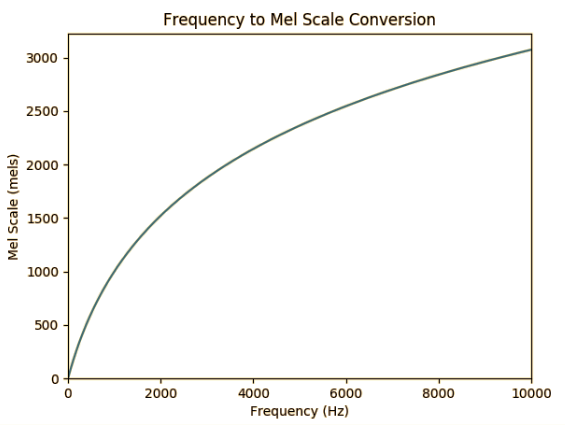
\includegraphics[width=0.5\linewidth]{figures/hz2mel.png}
	\caption{Conversion from frequency to mel scale}
	\label{fig:hz2mel}
\end{figure}

Initial feature extraction was done using the DCASE Challenge baseline system's included feature extractor, which makes use of python music and audio analysis package called LibROSA \cite{Heittola2017}. The feature extractor takes an audio file as an input and outputs an array in which each row is a time slice and each column is a feature, with the specifics dependent on a configurable parameters list. The parameters used can be seen in Table~\ref{tab:featExParam}.

Based on the settings used, the feature extractor output arrays with 501 time slices and 40 features, with each feature being the log of the magnitude of a band on the mel scale. This results in a feature set for each sound file of 20,040 dimensions.

\begin{table}
	\centering
	\caption{DCASE Baseline feature extractor parameters used}
	\label{tab:featExParam}
	\begin{tabularx}{0.76\textwidth}{l c}
		\toprule
		\textbf{Parameter}                           & \textbf{Value}     \\ \midrule
		Maximum frequency for calculating MEL band   & 22,050             \\
		Minimum frequency for calculating MEL band   & 0                  \\
		Sample frequency                             & 44,100             \\
		Hop length (samples)                         & 882                \\
		Hop length (seconds)                         & 0.02               \\
		Use htk style mel conversion                 & false              \\
		Use log scale                                & true               \\
		Feature extraction method                    & MEL                \\
		Average multichannel audio to single channel & true               \\
		FFT length                                   & 2,048              \\
		Number of MEL bands                          & 40                 \\
		Normalise MEL bands                          & false              \\
		Type of spectrogram                          & magnitude          \\
		Window length (samples)                      & 1764               \\
		Window length (seconds)                      & 0.04               \\
		Window type                                  & Hamming asymmetric \\ \bottomrule
	\end{tabularx}
\end{table}




\subsection{Feature Reduction}
\label{sec:featReduce}

The feature set extracted using the baseline system has a very high dimension, and in that form would be unsuitable for use with an LCS as a feature set of that size would cause increased processing time as well as classifiers that are overfitted to specific instances. In order to perform dimensionality reduction without losing too much important information about the datasets, some visualisations were made to facilitate identification of trends to potentially be exploited. Each of the graphs shown in Figure~\ref{fig:beachCarOffice} show the features extracted for a given sound file, with 9 different sound files of a given classification displayed together for the beach, car and office classifications. Each line represents one of the 501 time slices and the magnitude of each mel band in that slice. 

\begin{figure}[!htbp]
	\centering
	\begin{subfigure}[t]{0.54\textwidth}
		\centering
		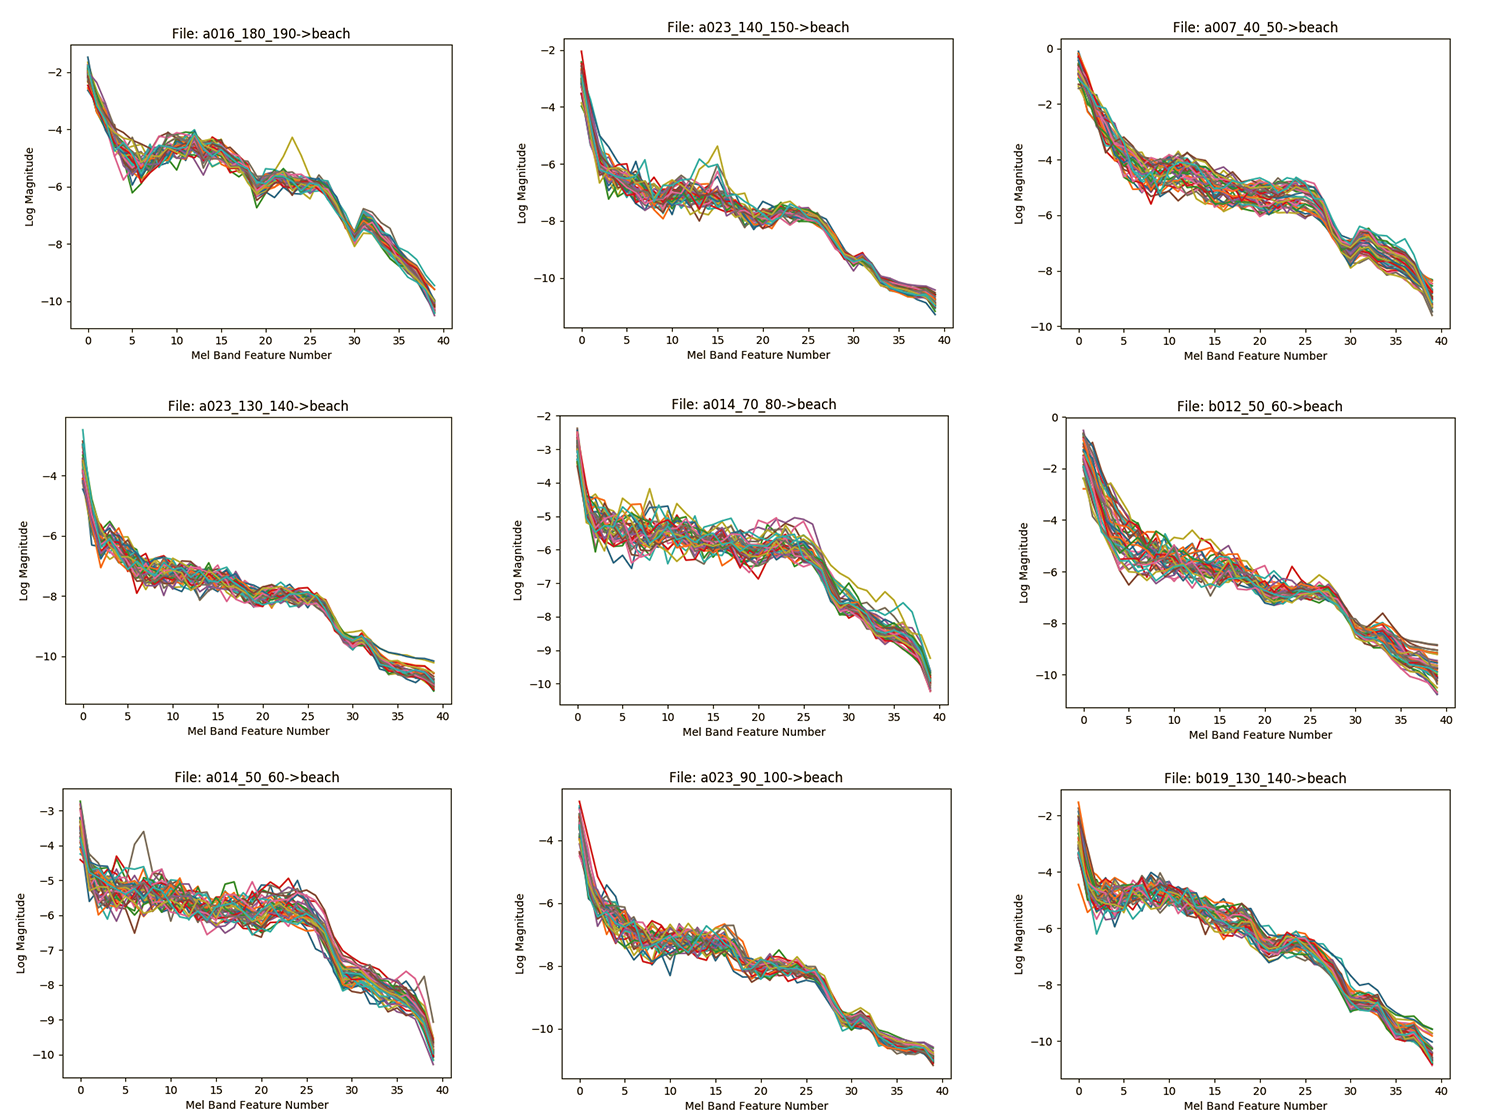
\includegraphics[width=0.9\textwidth]{figures/beachgrid.png}
		\caption{Beach}
	\end{subfigure}
	\\
	\vspace{0.2cm}
	\begin{subfigure}[t]{0.54\textwidth}
		\centering
		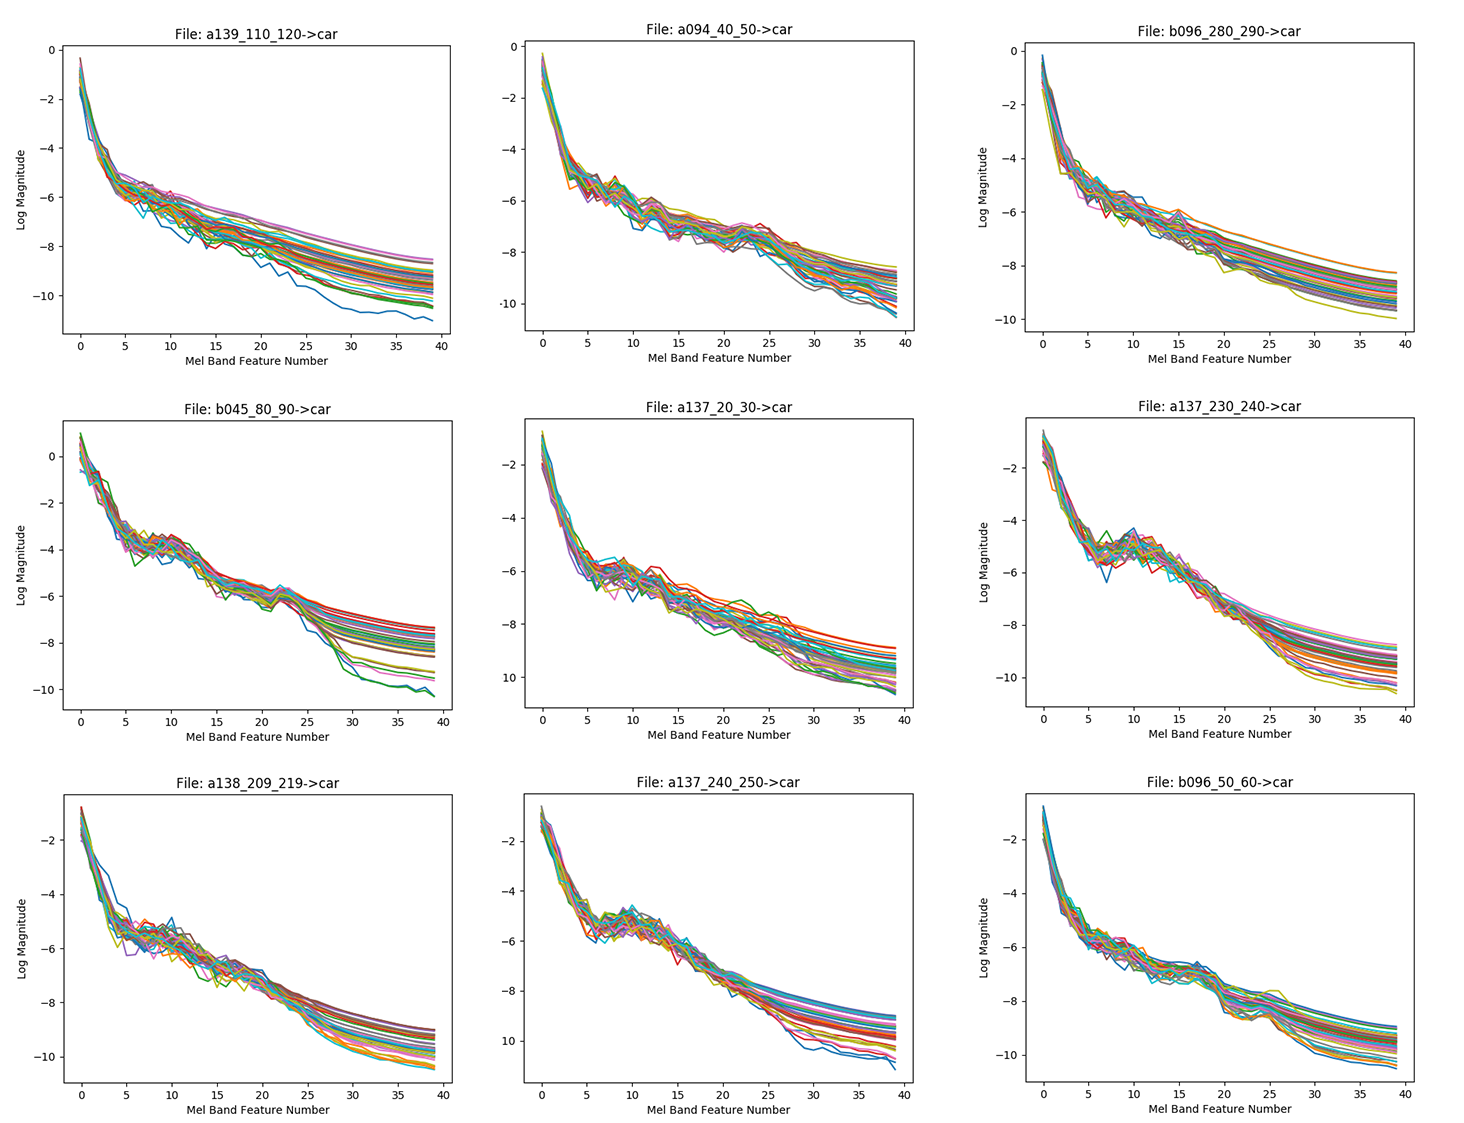
\includegraphics[width=0.9\textwidth]{figures/cargrid.png}
		\caption{Car}
	\end{subfigure}
	\\
	\vspace{0.2cm}
	\begin{subfigure}[t]{0.54\textwidth}
		\centering
		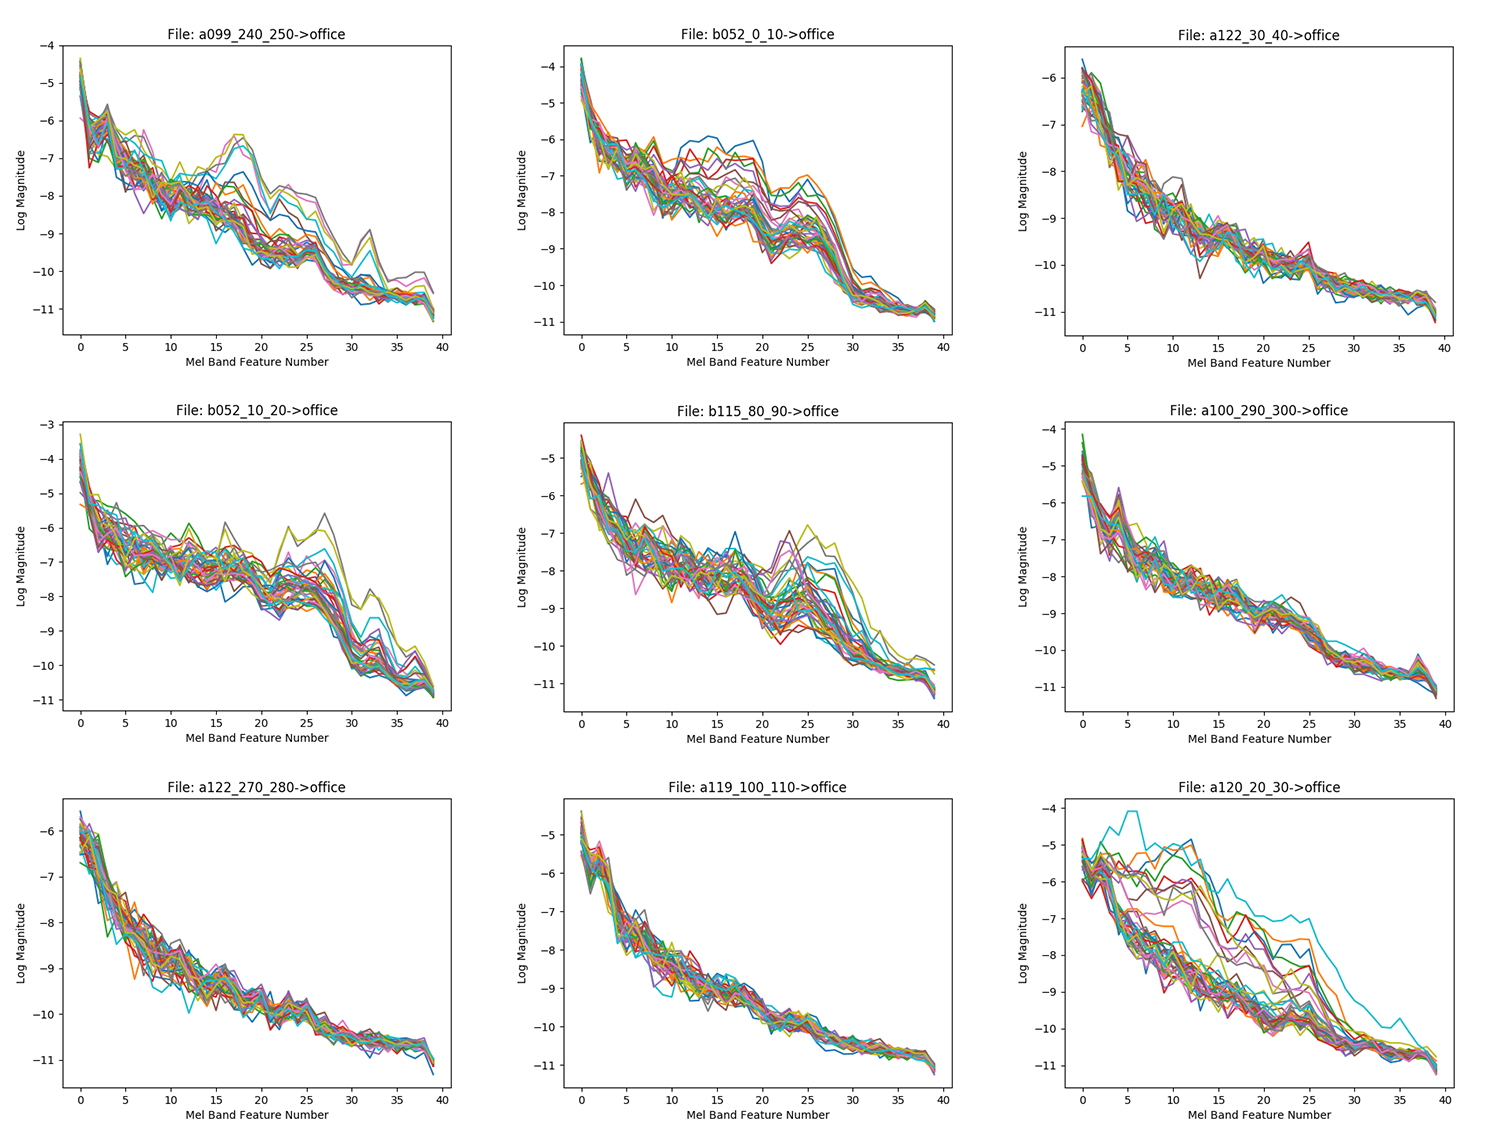
\includegraphics[width=0.9\textwidth]{figures/officegrid.png}
		\caption{Office}
	\end{subfigure}
	\caption{Extracted features for beach, car and office sound files}
	\label{fig:beachCarOffice}
\end{figure}

Comparing these graphs, it is clear that there are patterns common to individual classifications and that in a given sound file, the distribution of mel band magnitudes follows a similar pattern for many of the time slices. Given this similarity between time slices, it was decided that the mean and standard deviation of each mel band magnitude across all time slices would be used as the feature set, as this reduces the dimensionality by a factor of 250 while maintaining a measure of both the trend and spread of the data.

The three example classes shown in Figure~\ref{fig:beachCarOffice} are shown again in Figure~\ref{fig:beachCarOfficeAvg} with the difference that each line represents the \textit{average} log magnitude of for each mel band in one sound file of the given class, rather than each line being one time slice of a single file. These graphs illustrate that by taking the mean magnitude for each mel band, the general trends are preserved, and though the spreading of these values between time slices is not represented, it is captured in the standard deviations for each mel band. The average mean and standard per mel band across all sound files of each example classification is shown in Figure~\ref{fig:avgAndStd} and illustrates that the differences between classifications is still captured by the chosen features despite the extreme dimension reduction.

\begin{figure}[h]
	\centering
	\begin{subfigure}[t]{0.31\textwidth}
		\centering
		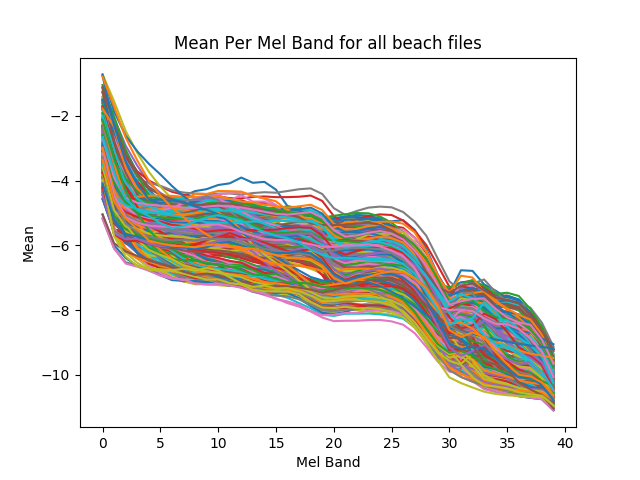
\includegraphics[width=\textwidth]{figures/beach.png}
		\caption{Beach}
	\end{subfigure}
	\begin{subfigure}[t]{0.31\textwidth}
		\centering
		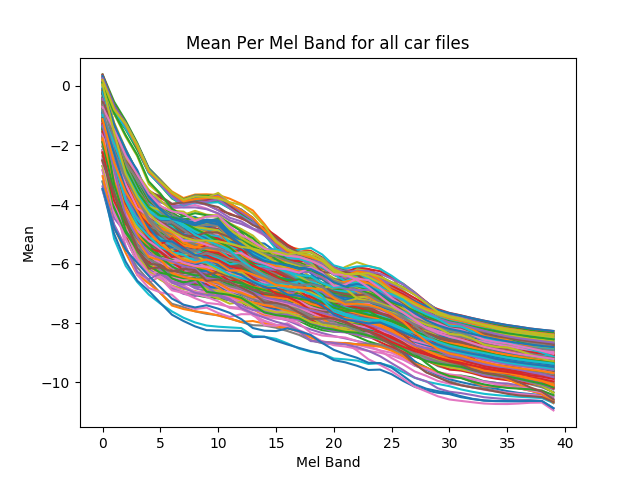
\includegraphics[width=\textwidth]{figures/car.png}
		\caption{Car}
	\end{subfigure}
	\begin{subfigure}[t]{0.31\textwidth}
		\centering
		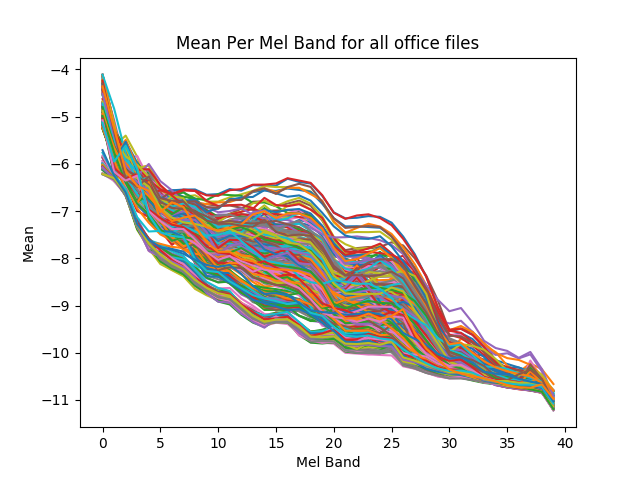
\includegraphics[width=\textwidth]{figures/office.png}
		\caption{Office}
	\end{subfigure}
	\caption{Average mel bands for each sound file in beach, car and office classifications}
	\label{fig:beachCarOfficeAvg}
\end{figure}

\begin{figure}[!htbp]
	\centering
	\begin{subfigure}[t]{0.48\textwidth}
		\centering
		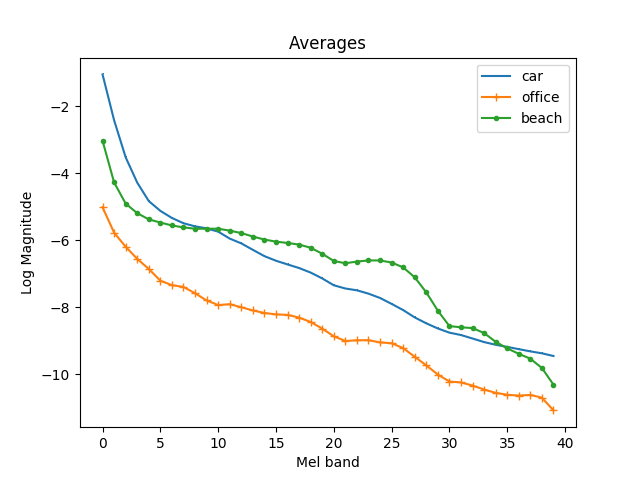
\includegraphics[width=0.9\textwidth]{figures/3Means.png}
		\caption{Means}
	\end{subfigure}
	\begin{subfigure}[t]{0.48\textwidth}
		\centering
		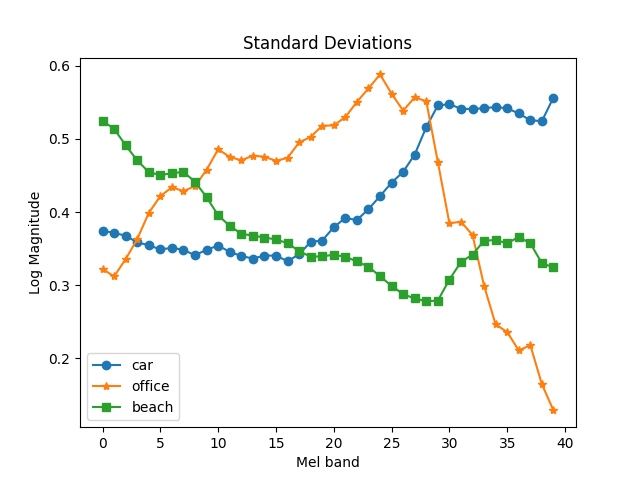
\includegraphics[width=0.9\textwidth]{figures/3Stds.png}
		\caption{Standard deviations}
	\end{subfigure}
	\caption{Average and standard deviation of sound file averaged mel bands across all sound files for a given classification}
	\label{fig:avgAndStd}
\end{figure}

The amount of spread between different instances of each class observed in Figure~\ref{fig:beachCarOfficeAvg} is noticeably large and would result in classifiers needing to have a large range of accepted values in order to catch many other instances of their classification. This spreading is potentially due to the sound files having different recorded volumes which may result in the magnitude offsets observed.

In attempting to rectify this, the means were normalised such that in a given sound file, instead of using the means as features, the average across the means of each mel band was taken and the features used were the mel band means subtract the average mean. This method would make magnitude offset irrelevant while maintaining trends and is illustrated in Figure~\ref{fig:norm} with the results of this transformation displayed in Figure~\ref{fig:beachCarOfficeVar} confirming that the general trends are preserved while reducing spread on the y axis.

Unfortunately, upon testing, this method was found to reduce classification accuracy so it was discontinued. Further analysis of the feature set showed that this is likely due to the offset of the mel band magnitudes being a defining characteristic of different scenes, which can be observed in Figure~\ref{fig:cmpOrigAndNorm} in which the average means of each class are plotted on one graph and the average normalised means are plotted on another. The graph of average means shows that classes are distinct from one another based on their magnitude offset and the other shows that by normalising them this discrimination is lost. The reduction in accuracy may imply that either the difference in trend was not enough to make classes distinct from one another or potentially that more parameter tuning of the LCS would be needed to take advantage of the normalisation.

\begin{figure}[!htbp]
	\centering
	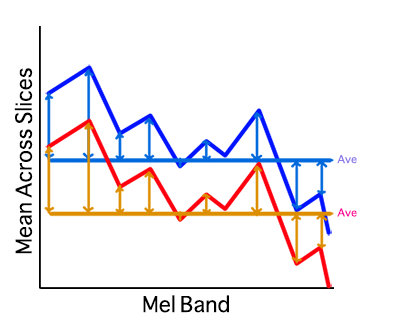
\includegraphics[width=0.5\linewidth]{figures/normalise.png}
	\caption{Normalisation procedure for feature data}
	\label{fig:norm}
\end{figure}

\begin{figure}[h]
	\centering
	\begin{subfigure}[t]{0.31\textwidth}
		\centering
		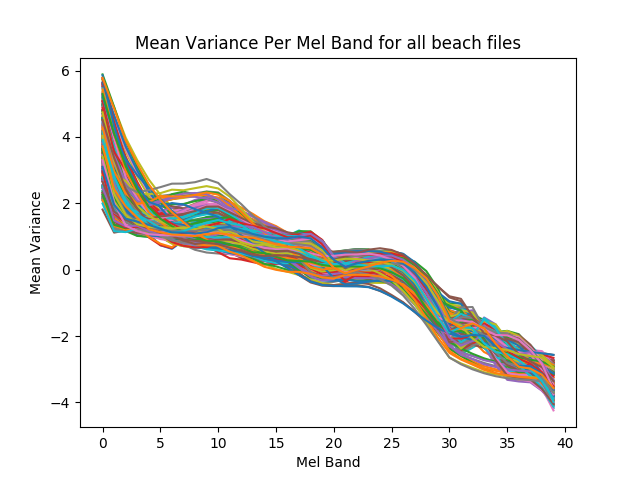
\includegraphics[width=\textwidth]{figures/beachVar.png}
		\caption{Beach}
	\end{subfigure}
	\begin{subfigure}[t]{0.31\textwidth}
		\centering
		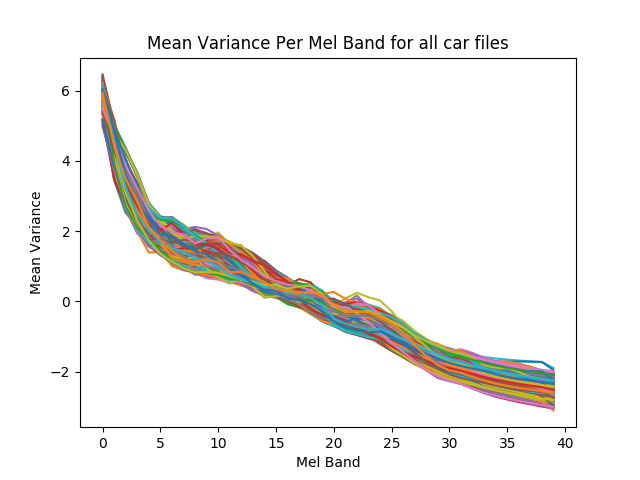
\includegraphics[width=\textwidth]{figures/carVar.png}
		\caption{Car}
	\end{subfigure}
	\begin{subfigure}[t]{0.31\textwidth}
		\centering
		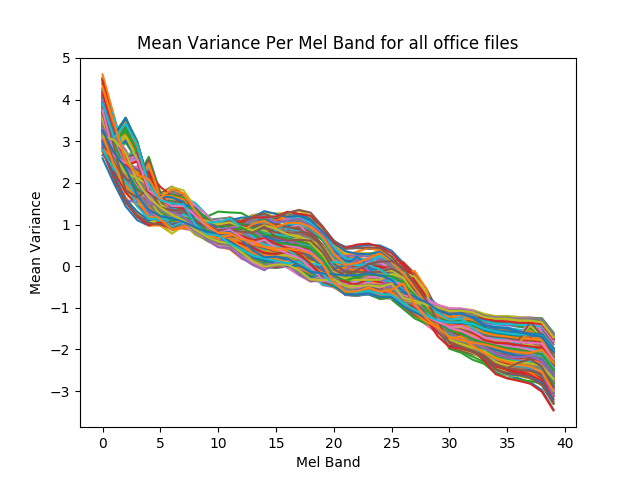
\includegraphics[width=\textwidth]{figures/officeVar.png}
		\caption{Office}
	\end{subfigure}
	\caption{Normalised mean mel band values for each sound file in each classification shown}
	\label{fig:beachCarOfficeVar}
\end{figure}

\begin{figure}[!htbp]
	\centering
	\begin{subfigure}[t]{0.48\textwidth}
		\centering
		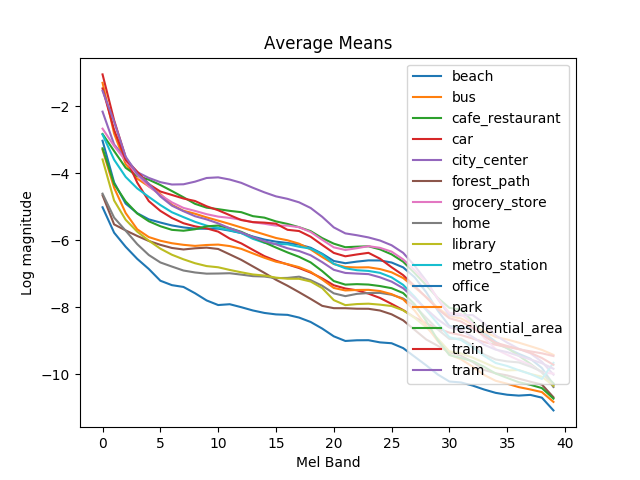
\includegraphics[width=0.9\textwidth]{figures/allMeans.png}
		\caption{Means}
	\end{subfigure}
	\begin{subfigure}[t]{0.48\textwidth}
		\centering
		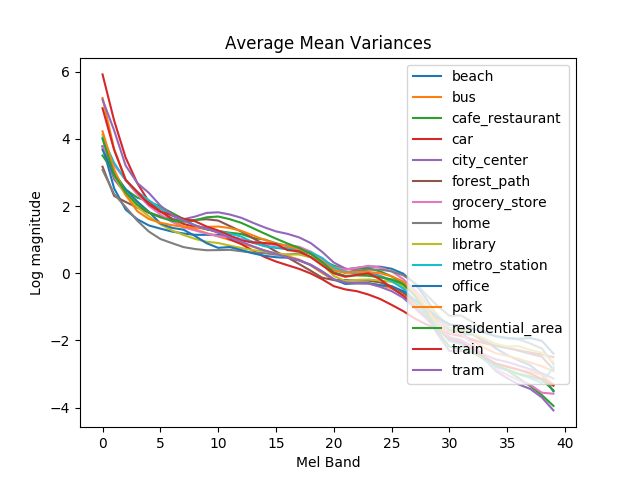
\includegraphics[width=0.9\textwidth]{figures/allMeanVars.png}
		\caption{Standard deviations}
	\end{subfigure}
	\caption{Comparison of original and normalised mel band averages across each classification}
	\label{fig:cmpOrigAndNorm}
\end{figure}







\section{Experiment 1: Baseline System}
\label{sec:exp1}

An investigation into LCSs built by others led us to sourcing from a sample system hosted on GitHub titled eLCS [?]. This Michigan-style classifier created by R. J. Urbanowicz [?] was developed as an educational tool that demonstrated the intricacies and components that contribute towards building a typical LCS. It consists of five demo folders showing the steps towards building a typical LCS and a dataset consisting of discrete attributes and a starting rule population to run the LCS. For our purposes, we used the last folder `Demo 5' as the starting point for constructing our LCS. This was used for the initialisation of the Github repository used for this experiment [?].

Preliminary steps towards understanding the functional processes of this LCS included refactoring and inserting comments while stepping through the code using a debugging process. From this it was discovered early in the process that the LCS had support for continuous values for attributes and could be initialised without a predefined rule population. These features which were not apparent during our project introduction presentati, greatly simplified the process of adapting our dataset to work with this implementation of an LCS. Other results from these works included: refactoring the LCS code to a submodule, creation of a `utils' directory for preprocessing of feature files, creation of a `notebooks' directory for visualising the results and a `docs' directory for holding compiled documentation files. PDF generated documentation can be found at the root level of the repository.

In order to utilize the dataset processed by the libROSA library in the DCASE baseline solution, further processing of this dataset needed to take place to make it suitable for our implementation. As the dataset was too large for importation into our LCS model, the first approach was to reduce its dimensionality by calculating the mean and standard deviation over the time series data. When calculated over the entire range, it reduced the size of the dataset by a factor of 256:1. Other approaches included dividing the time series data into even slices and calculating the mean and standard deviation on these individual segments. After applying this process the dataset was then optionally split into training and testing datasets of varying ratios, ensuring that an even number of features were maintained in each dataset.

\begin{table}
	\caption{LCS Baseline models using Training data only}
	\label{lcs-bs-models-tr}
	\begin{tabular}{|l|l|l|l|}
		\hline
		Model & Segments & Population Size & Maximum Iterations \\ \hline
		1 & 1 & 1,000 & 500,000 \\
		2 & 8 & 1,000 & 500,000 \\
		3 & 1 & 3,000 & 30,000 \\
		3 & 1 & 5,000 & 50,000 \\
		\hline
	\end{tabular}
\end{table}

For the first series of simulations the entire training dataset (4680 instances) was used to generate the rule population for feature prediction without any testing data. Although this results in a grossly overfit prediction model, it seeks to determine the performance of the LCS to generate rule populations that are able to correctly classify elements in the training dataset. The models generated in this section are listed in Table ??

\todo[inline]{---bs-plot-1.png here---}

Figure ?? shows a comparison of Models 1 and 2 in which we evaluate the rule population accuracy with an increase in the number of segments to the time series data. These simulations were also run for a large number of iterations to evaluate how accuracy changed with time. A comparison of these models has shown that a strong correlation between segmentation size and population rule accuracy. It also showed that running the model for an extended period of time had no bearing on increasing its accuracy. Model 1 was shown to have benefit from running up until approximately 100,000 iterations, while Model 2 had no benefit at all.

\todo[inline]{---bs-plot-2.png here---}

Figure ?? shows a comparison of Models 1, 3 and 4 in which we evaluate the rule population accuracy with an increase to the population size up to a maximum of 50,000 iterations. These results showed that a strong correlation existed between population size and population rule accuracy. It should be noted however that increasing the population size also resulted in a substantial increase to computation time.



\section{Experiment 2: Custom LCS Implementation}
\label{sec:exp2}

In response to the positive results obtained from the baseline system described above, a separate LCS algorithm was coded by the authors. This provided much greater ability to control various aspects of the algorithm and more clarity as to the overall system's functioning. This section presents the general approach to developing this algorithm (Section~\ref{sec:exp2appr}), a description of each of the key parameters (Section~\ref{sec:exp2params}) and the key modifications made to the standard LCS design (Section~\ref{sec:exp2mods}).





\subsection{Overview of Approach}
\label{sec:exp2appr}

The LCS algorithm developed by the authors was closely based on the structure and pseudocode provided by \citeauthor{Butz2000} in their paper entitled ``An Algorithmic Description of LCS'' \cite{Butz2000}. This paper provides detailed descriptions for each of the key modules of XCS, which is one of the most well-regarded LCS implementations \cite{Sigaud2007}. The decision to embark on developing a custom LCS implementation was largely based on the availability of the pseudocode in this paper.

Two fundamental changes made to the algorithm presented by \citeauthor{Butz2000} were the change to continuous data, and hence continuously-valued classifier rules, and the switch from reinforcement learning to offline learning. Both changes necessitated a significant number of alterations throughout the algorithm. Various papers were consulted for how to make these changes. In particular, a number of papers on XCSR -- the standard continuous data version of XCS -- were referenced~\cite{Sowden2007,Stone2003,Wilson2000,Behdad2012}.

Continuous valued rules were implemented using the centre-range encoding \cite{Sowden2007}. In this scheme, each rule within a classifier's condition matches values between centre - range and centre + range. Note that this representation, and indeed any continuous representation, doubles the number of ``alleles'' in a classifier with two for each rule \cite{Sowden2007}.

Additionally, the GA required a number of design decisions. These included the use of two-point crossover, roulette-wheel parent selection and employing GA subsumption (where parents can subsume children if they are more general). The GA was also applied in a `niched' manner to act only on the correct set. Niched GA operation has been noted as a significant contributor to LCS performance \cite{Lanzi2008}. Accuracy-based fitness, another key performance enhancing feature \cite{Lanzi2008}, was also used.

As discussed in Section~\ref{sec:featReduce}, the mean and standard deviation of log mel bands were used as the features for each sound file in this experiment. All 312 sound files from all of the 15 sound contexts were considered. That is, the LCS \textit{environment} consisted of 312 \textit{instances} (sound files) per \textit{endpoint} (context), giving a total of 4,680 instances, each containing 80 \textit{attributes} (features; 40 means, 40 standard deviations). Data was split into training and testing datasets with a 60:40 ratio.







\subsection{Parameters}
\label{sec:exp2params}

\todo[inline]{Import Yiyang's section}






\subsection{Problem-Specific Modifications}
\label{sec:exp2mods}

Four components of the custom LCS implemented here required appreciable modification from standard practice. First, in designing the mutation scheme for the continuously-valued rules, it was desired to allow for each possible case. That is, mutation from specific values to wildcards, wildcards to specific values and specific values to other specific values. The methods used for each case are listed in Table~\ref{tab:mutMeth}. Note mutation may occur independently on any rule centre \textit{or} range value independently, with the exception that a given centre-range pain must either both be specific values or both be wildcards; never can one be a wildcard and the other not.

\begin{table}[!htbp]
	\centering
	\caption{Mutation methods}
	\label{tab:mutMeth}
	\begin{tabularx}{0.9\textwidth}{l p{9cm}}
		\toprule
		\textbf{Mutation type}           & \textbf{Mutation method}                                                                            \\ \midrule
		Specific value to wildcard       & Substitute associated centre \textit{and} range with wildcards (`\#')                                         \\
		Wildcard to specific value       & Set associated centre \textit{and} range to value from current instance from environment plus a random, randomly signed increment \\
		Specific value to specific value & Add a random, randomly signed increment                                                             \\ \bottomrule
	\end{tabularx}
\end{table}

Table~\ref{tab:mutProb} lists the probabilities of various quantities of alleles being mutated in a given classifier based on a mutation probability of 0.02, which is relatively standard \cite{Butz2000}. As shown, there is a slightly less than 4\% chance that mutation will not affect a given child. Combined with the probability of covering being set to 0.7 (also within the range of standard values \cite{Butz2000}), this means that there is a 2.7\% chance of a given child classifier being identical to its parent (in which case it will obviously be subsumed).

\begin{table}[!htbp]
	\centering
	\caption{Mutation probabilities}
	\label{tab:mutProb}
	\begin{tabularx}{0.3\textwidth}{cc}
		\toprule
		\textbf{Quantity} & \textbf{Probability} \\ \midrule
		        0         &         0.04         \\
		        1         &         0.13         \\
		        2         &         0.21         \\
		        3         &         0.24         \\
		        4         &         0.18         \\
		        5         &         0.11         \\
		     $\ge$ 6      &         0.10         \\ \bottomrule
	\end{tabularx}
\end{table}

Second, as per standard practice, correct set subsumption was used in this implementation; however, a different metric for determining the most general classifier in the correct set wa required \cite{Butz2000}. In XCS, the metric is to simply choose the classifier with the greatest number of wildcards. In this implementation, and additional criteria was added so that if more than one classifier has the equal most wildcards, the classifier with the largest total range is selected as the most general. This does not appear to be standard practice, but does fit intuitively.

Third, the conditions for one classifier to subsume another were drastically relaxed. This was motivated by the fact that subsumption, which is critical to evolving maximally general classifiers, was not occurring. The explanation for this is simply that it is extremely unlikely.

Consider the standard criteria for a classifier to be ``more general'' than another. To do so, its rule intervals must cover that of the classifier it is proposing to subsume for \textit{all} attributes and, if the proposed subsumee has a wildcard at \textit{any} attribute, the proposed subsumer must also have a matching wildcard \cite{Sowden2007,Wilson2000}.

With the parameters used in this LCS implementation, the probability of a given rule being a wildcard is approximately 0.15. Hence, the probability of a proposed subsumee having a wildcard where the subsumer does not at any given attribute is 0.15~x~0.85 = 0.128. Across 80 rules, this means that there there is only a 1 in 55,000 chance that a subsumption match is possible. However, this analysis does not even take into account the criteria for the subsumer to have superior ranges than its subsumee, so this is actually an upper bound on the true probability.

To remedy this, the criteria for the subsumer to match each wildcard in the subsumee has been removed and a tolerance has been added to the interval matching criteria. That is, a classifier can still be said to be more general than another if its rule interval, when expanded by some tolerance factor, covers the other rule. Overall, this represents a weak form of subsumer generality that does not appear to be used in the literature. However, the authors would suggest that modifications of this nature are essential to ensuring subsumption can occur in problems with large numbers of attributes and continuous data.

Fourth, the experience threshold for deletion of a classifier from the population has been made dependent on the classifier's age. This was motivated by the observation that many classifiers require many iterations to reach the standard threshold for candidacy for deletion (a match count of at least 20). As a result, as soon as any classifiers do reach it they are very likely to be deleted since they are the only classifiers eligible for deletion. However, this is undesired as these are often reasonably well-performing classifiers.

Consequently, the authors devised an alternative deletion experience threshold that rolls off after a specified age (number of iterations since the classifier's birth). The rule for this threshold is defined by the following equation and illustrated in Figure~\ref{fig:deletionthreshold}
\[
	\frac{\textrm{exp}_{min}}{3.05}
	\left(
	\pi/2-\arctan\left(\frac{\textrm{age} - \textrm{age}_{min}}{20} \right) \right)
\]
Where $exp_{min}$ is the initial minimum experience threshold (that will apply to new classifiers), age is the number of iterations since the classifier's birth and $age_{min}$ is the threshold age after which the experience threshold drops off substantially.

\begin{figure}[!htbp]
	\centering
	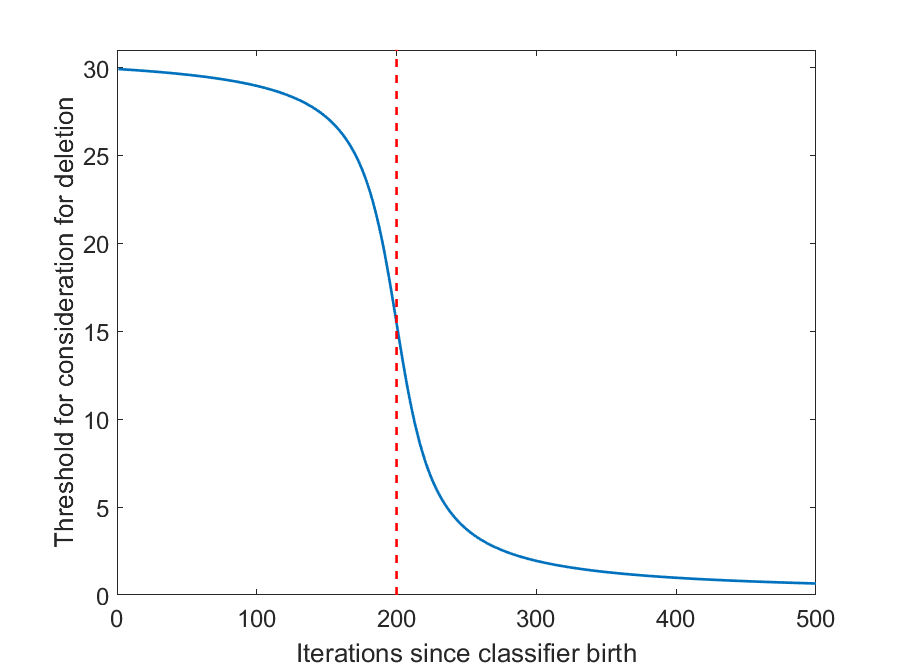
\includegraphics[width=0.7\linewidth]{figures/deletionThreshold.png}
	\caption{Variable deletion threshold with cut-off age depicted as dashed vertical red line}
	\label{fig:deletionthreshold}
\end{figure}



\section{Results}

\todo[inline]{Yiyang: feel free to mess around with the sub-headings under Results if you wish}




\subsection{Environment Representations}

Alternative feature processing investigated



\subsection{Parameter Tuning}

%- Rate of learning (improvement in accuracy over time)
%
%- Overall results: pairwise, all classes at once (confusion matrices)
%
%
%Theoretical analysis?



Reason why standard deviation and mean are used, what information they carry


Car and office confusion matrix
Plot for std dev and mean (for car and office) to explain
Car, office and city centre (with confusion and plots)
Then add metro station and show results (worse) - explain why it is worse
Show a classifier on a graph to show how it can match instances
Overall accuracy (all 15 features)


\section{Discussion}


Our approach is good because it is more general (no need to construct statistical models or decision rules) and significantly reduces the number of features that need to be analysed, and therefore the complexity of the algorithm. [THIS IS COMPARING TO STANDARD APPROACH TO ACS / DCASE CHALLENGE SUBMISSIONS]







\section{Future Research}

As previously discussed, quality of the results achieved by a machine learning system is highly dependent on the quality of the features used as input. While reducing the dimension of the data by taking the mean and standard deviation of the mel bands worked well for classification of a few different scenes, the classifier performed poorly when presented with more categories to discriminate. This behaviour indicates that the features used did not adequately capture the nuances separating different scenes and that representing the data in different ways may be beneficial to performance.
It may be useful to do Fourier analysis in order to better represent the shape of a sound file's magnitude-mel band curve, as the shape appears to be a distinctive feature for many of the instances. While this could be useful, more research would be needed to determine a means of representing a Fourier series in a way that doesn't increase dimensionality too drastically. 
The DCASE Baseline system provides numerous different ways of extracting features from sounds files, so another avenue of future research would be to test the performance of different types of features extractable with the system. Potential experiments could be conducted into making use of mel scale cepstral coefficients rather than pure mel scale band data as well as experimenting with different window lengths, hop lengths and mel band sizes. A neural network or genetic algorithm could be used to optimise the feature extraction as well as LCS parameters in order to find the optimal settings across both systems. 
Smoothness of the different magnitude-mel band curves would be an interesting feature to look into using for future experiments. Features could potentially be derived from the location of maxima and minima as well as the smoothness between adjacent mel bands.
There might also be potential for research into swapping the data and plotting the magnitude over time of each mel band. Upon inspection, patterns do not immediately emerge as with magnitude over mel band of each time slice, but further research may find significant features to be extracted from that data. Example plots of magnitude over time for different mel bands can been seen in 
\todo[inline]{flipItBoyo.png}
Given time for further research, investigation into classification using the high dimensional data directly extracted using the DCASE Baseline system's feature extractor also has potential to yield better results. Retaining all of the time data would make classifiers in the LCS more prone to overfitting an instance, but increasing generality with a higher proportion of wildcards may be able to offset this while also allowing useful information to be exploited rather than lost. This would also require a larger training dataset in order to be properly tested, as more data points would be needed to describe the higher dimensional space.

\section{Conclusion}
Acoustic sound classification is ongoing field of research in which machine learning techniques have recently been making fast progress. The annual Detection and Classification of Acoustic Scenes and Events (DCASE) challenge provides various sound related tasks for competitors to train models on in attempts to push the boundaries of machine sound recognition performance. The challenge provides a training data set of sound files as well as a Baseline system that performs feature extraction by decomposing audio data into useable features. Taking a different direction to the neural networks that are most commonly used in this competition, learning classifier systems (LCSs) were used to explore their suitability to the given task of acoustic scene classification. Using the feature extractor provided, a feature set comprised of the average magnitude for 40 mel bands over the sound files was used to train the LCSs. It was found that while the system would perform extremely well when discriminating between a small set a classes, performance declined steeply as the number of classes increased and the patterns characterising them become less distinctive. It is potentially due to the method of dimension reduction used that the LCSs’ struggled to discriminate between larger sets of classes, so further research is required to investigate alternative feature sets and matching LCS parameters settings that may allow the systems to achieve greater performance in this area.


\bibliographystyle{IEEEtranN}
\bibliography{IEEEabrv,References}

%\end{multicols}

\end{document}